%! alt A regular dodecagon ABCDEFGHIJKL with centre O. The rectangle ABGH is shaded, with its short side AB a side of the dodecagon and its diagonals AG and BH diameters through O. The segments OA, OB, OG and OH cut it into four triangles: OAB and OGH have a 30 degree angle at O, and OBG and OHA have a 150 degree angle at O. Each of the four has area 30, the same as each of the twelve central triangles, so the rectangle has area 120.
%! after_paragraph 1
%! scale 3/10
%! let R = sqrt(120)
% The shared preamble of every Cevian figure. pipeline/figures turns these colours into theme-aware paint,
% and refuses any other colour, so draw only with them:
%   figink (lines and labels), figaux (construction lines), figaccent (the object the argument turns on),
%   figtint and figaccenttint (light fills).
\documentclass[border=1.5pt]{standalone}
\usepackage{tkz-euclide}
\definecolor{figink}{RGB}{0,0,0}
\definecolor{figaux}{RGB}{85,85,85}
\definecolor{figaccent}{RGB}{192,57,43}
\definecolor{figtint}{RGB}{221,221,221}
\definecolor{figaccenttint}{RGB}{245,213,208}
% tkz-euclide's defaults draw circles, compasses and marks in 50% grey and fill points with a tint.
\makeatletter
\def\tkz@otherlinecolor{figink}
\def\tkz@euc@circlecolor{figink}
\def\tkz@euc@compasscolor{figink}
\def\tkz@euc@mkcolor{figink}
\def\tkz@mk@fill{figink}
\def\tkz@euc@pointfillcolor{figink}
\makeatother
\tkzSetUpLine[color=figink,line width=.7pt]
\tkzSetUpArc[color=figink,line width=.7pt]
\tkzSetUpCompass[color=figink,line width=.5pt]
\tkzSetUpPoint[color=figink,fill=figink,size=3.1pt]
\tikzset{
  every picture/.style={line cap=round,line join=round,color=figink},
  circle style/.append style={color=figink,line width=.7pt},
  aux/.style={color=figaux,line width=.45pt,dash pattern=on 2.6pt off 2pt},
  key/.style={color=figaccent,line width=1pt},
  mk/.style={color=figink,line width=.5pt},
  lbl/.style={color=figink,inner sep=2.2pt},
  len/.style={color=figink,inner sep=1.5pt,font=\small},
}

\begin{document}
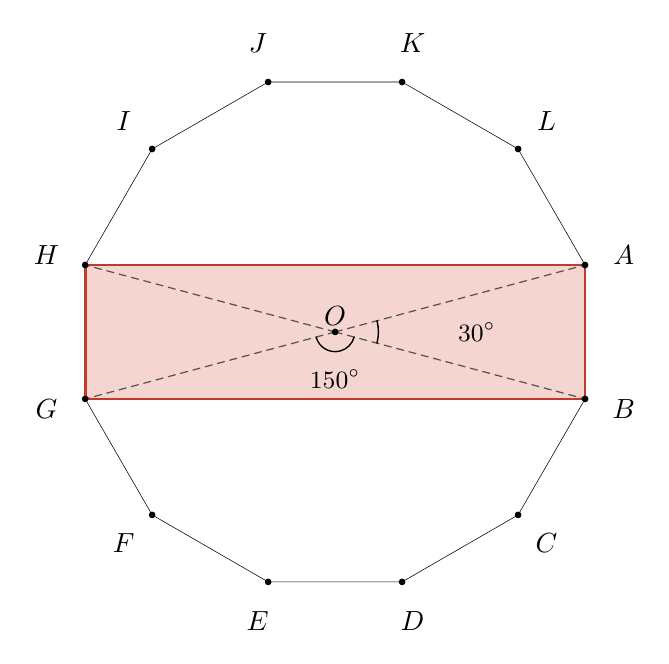
\begin{tikzpicture}
\tkzDefPoint(0.0,0.0){O} %! O = (0, 0)
\tkzDefPoint(3.1743562,0.85056618){A} %! A = polar(O, R, 15)
\tkzDefPoint(3.1743562,-0.85056618){B} %! B = polar(O, R, -15)
\tkzDefPoint(2.3237900,-2.3237900){C} %! C = polar(O, R, -45)
\tkzDefPoint(0.85056618,-3.1743562){D} %! D = polar(O, R, -75)
\tkzDefPoint(-0.85056618,-3.1743562){E} %! E = polar(O, R, -105)
\tkzDefPoint(-2.3237900,-2.3237900){F} %! F = polar(O, R, -135)
\tkzDefPoint(-3.1743562,-0.85056618){G} %! G = polar(O, R, -165)
\tkzDefPoint(-3.1743562,0.85056618){H} %! H = polar(O, R, -195)
\tkzDefPoint(-2.3237900,2.3237900){I} %! I = polar(O, R, -225)
\tkzDefPoint(-0.85056618,3.1743562){J} %! J = polar(O, R, -255)
\tkzDefPoint(0.85056618,3.1743562){K} %! K = polar(O, R, -285)
\tkzDefPoint(2.3237900,2.3237900){L} %! L = polar(O, R, -315)
\tkzDefPoint(3.6669784,0.98256389){LA} %! LA = polar(O, R + 1.7, 15)
\tkzDefPoint(3.6669784,-0.98256389){LB} %! LB = polar(O, R + 1.7, -15)
\tkzDefPoint(2.6844145,-2.6844145){LC} %! LC = polar(O, R + 1.7, -45)
\tkzDefPoint(0.98256389,-3.6669784){LD} %! LD = polar(O, R + 1.7, -75)
\tkzDefPoint(-0.98256389,-3.6669784){LE} %! LE = polar(O, R + 1.7, -105)
\tkzDefPoint(-2.6844145,-2.6844145){LF} %! LF = polar(O, R + 1.7, -135)
\tkzDefPoint(-3.6669784,-0.98256389){LG} %! LG = polar(O, R + 1.7, -165)
\tkzDefPoint(-3.6669784,0.98256389){LH} %! LH = polar(O, R + 1.7, -195)
\tkzDefPoint(-2.6844145,2.6844145){LI} %! LI = polar(O, R + 1.7, -225)
\tkzDefPoint(-0.98256389,3.6669784){LJ} %! LJ = polar(O, R + 1.7, -255)
\tkzDefPoint(0.98256389,3.6669784){LK} %! LK = polar(O, R + 1.7, -285)
\tkzDefPoint(2.6844145,2.6844145){LL} %! LL = polar(O, R + 1.7, -315)
\tkzDefPoint(1.8000000,0.0){Q} %! Q = polar(O, 6, 0)
\tkzDefPoint(0.0000000000000000000000000000000000000000000000000013004501,-0.60000000){S} %! S = polar(O, 2.0, -90)
%! fact area(A, B, C, D, E, F, G, H, I, J, K, L) == 360
%! fact area(O, A, B) == 30
%! fact area(O, B, G) == 30
%! fact angle(A, O, B) == 30
%! fact angle(B, O, G) == 150
%! fact area(A, B, G, H) == 120
%! fact collinear(O, A, G)
%! fact collinear(O, B, H)
\tkzFillPolygon[color=figaccenttint](A,B,G,H)
\tkzDrawPolygon(A,B,C,D,E,F,G,H,I,J,K,L)
\tkzDrawPolygon[key](A,B,G,H)
\tkzDrawSegments[aux](O,A O,B O,G O,H)
\tkzMarkAngle[size=.55,arc=l,mark=none,mk](B,O,A)
\tkzMarkAngle[size=.25,arc=l,mark=none,mk](G,O,B)
\tkzLabelPoint[anchor=center,font=\small](Q){$30^\circ$}
\tkzLabelPoint[anchor=center,font=\small](S){$150^\circ$}
\tkzDrawPoints(O,A,B,C,D,E,F,G,H,I,J,K,L)
\tkzLabelPoint[above,lbl](O){$O$}
\tkzLabelPoint[anchor=center,lbl](LA){$A$}
\tkzLabelPoint[anchor=center,lbl](LB){$B$}
\tkzLabelPoint[anchor=center,lbl](LC){$C$}
\tkzLabelPoint[anchor=center,lbl](LD){$D$}
\tkzLabelPoint[anchor=center,lbl](LE){$E$}
\tkzLabelPoint[anchor=center,lbl](LF){$F$}
\tkzLabelPoint[anchor=center,lbl](LG){$G$}
\tkzLabelPoint[anchor=center,lbl](LH){$H$}
\tkzLabelPoint[anchor=center,lbl](LI){$I$}
\tkzLabelPoint[anchor=center,lbl](LJ){$J$}
\tkzLabelPoint[anchor=center,lbl](LK){$K$}
\tkzLabelPoint[anchor=center,lbl](LL){$L$}
\end{tikzpicture}
\end{document}
